\documentclass[aspectratio=169,11pt]{beamer}
\usepackage[utf8]{inputenc}
\usepackage[T1]{fontenc}
\usepackage[brazil]{babel}
\usepackage{lmodern}
\usepackage{booktabs}
\usepackage{amsmath,amssymb}
\usepackage{graphicx}

% ---------------- aparência acadêmica: sóbria, serifada, sem enfeite ----------
\usetheme{default}
\useoutertheme{infolines}
\usefonttheme{serif}
\setbeamertemplate{navigation symbols}{}
\setbeamertemplate{headline}{}

\definecolor{azulacad}{RGB}{20,50,90}
\definecolor{cinzafraco}{RGB}{100,100,100}

\setbeamercolor{structure}{fg=azulacad}
\setbeamercolor{frametitle}{fg=azulacad}
\setbeamercolor{title}{fg=azulacad}
\setbeamercolor{author}{fg=black}
\setbeamercolor{institute}{fg=cinzafraco}
\setbeamercolor{date}{fg=cinzafraco}
\setbeamercolor{itemize item}{fg=azulacad}
\setbeamercolor{itemize subitem}{fg=azulacad}
\setbeamercolor{palette primary}{fg=white,bg=azulacad}
\setbeamercolor{palette secondary}{fg=white,bg=azulacad}
\setbeamercolor{palette tertiary}{fg=white,bg=azulacad}

\setbeamerfont{frametitle}{series=\bfseries,size=\large}
\setbeamerfont{title}{series=\bfseries,size=\LARGE}
\setbeamerfont{subtitle}{series=\mdseries,size=\normalsize,shape=\itshape}
\setbeamerfont{footline}{size=\tiny}

% título de quadro com filete fino embaixo, no lugar da barra colorida
\setbeamertemplate{frametitle}{%
  \vskip0.9em%
  \usebeamerfont{frametitle}\usebeamercolor[fg]{frametitle}\insertframetitle%
  \vskip0.25em%
  {\color{azulacad}\hrule height0.5pt}%
  \vskip0.2em%
}

\setbeamertemplate{itemize item}{\textbullet}
\setbeamertemplate{caption}{\insertcaption}
\setbeamersize{text margin left=1.1em,text margin right=1.1em}

\graphicspath{{figuras/}}

\title[Peso de ações nos fundos brasileiros]%
      {Peso de ações nos fundos de investimento brasileiros}
\subtitle{Um modelo de fator dinâmico com correção logística e ajuste parcial}
\author[J. P. Zangrandi]{João Paulo Zangrandi}
\institute[FGV EESP]{Escola de Economia de São Paulo, Fundação Getulio Vargas\\[0.4em]
Orientador: Prof.\ Maurício Ferraresi Junior}
\date[2026]{2026}

\begin{document}

% ---------------------------------------------------------------- 1
{\setbeamertemplate{footline}{}
\begin{frame}[plain]
  \titlepage
\end{frame}}

% ---------------------------------------------------------------- 2
\begin{frame}{A pergunta, e a base para respondê-la}

A carteira divulgada de um fundo é demanda revelada. Olhando todos os fundos que carregam
a mesma ação no mesmo mês, o preço é comum a todos, e o que resta para explicar a diferença
entre eles são características dos próprios fundos.

\vspace{0.5em}
Duas perguntas: o que explica o peso, e esse peso é previsível fora da amostra.

\vspace{1.0em}
\centering
\small
\begin{tabular}{@{}lrrr@{}}
\toprule
& Fundos & Ativos & Gestoras \\
\midrule
Universo bruto CVM com posição em ações, 2016 a 2021 & 3.254 & 536 & 41 \\
Amostra final, com as seis características completas & 2.507 & 512 & 41 \\
\bottomrule
\end{tabular}

\vspace{0.9em}
\raggedright
\normalsize
8.212.294 observações de fundo por ativo e por mês, em 59 meses. Dado inteiramente público
da CVM, e o universo inteiro, não um recorte de uma gestora ou de um papel.

\vspace{0.5em}
\footnotesize
Referência: Koijen e Yogo (2019). O trabalho fica do lado das quantidades, não dos preços.

\end{frame}

% ---------------------------------------------------------------- 3
\begin{frame}{Etapa 1: o corte transversal}

Para cada ativo $n$ e cada mês $t$, uma regressão logística do peso nas características do
fundo $i$, estimada separadamente em cada célula:
\begin{equation*}
\text{peso}_{i,n,t} = g\big(x_{i,n,t}'\theta_{n,t}\big) + e_{i,n,t},
\qquad g(z)=\frac{1}{1+e^{-z}},
\qquad e_{i,n,t} = \text{peso}_{i,n,t} - g\big(x_{i,n,t}'\theta_{n,t}\big)
\end{equation*}

Seis características em $x_{i,n,t}$: tamanho, cotistas, fundo de cotas, fluxo sobre
patrimônio, beta da cota e a concentração do restante da carteira, definida como

\begin{equation*}
\text{HHI}_{\text{resto},i,n,t} = \text{HHI}_{\text{total},i,t-1} - \text{peso}_{i,n,t-1}^2,
\qquad
\text{HHI}_{\text{total},i,t-1} = \sum_{m} \text{peso}_{i,m,t-1}^2
\end{equation*}

\small
Subtrair $\text{peso}_{i,n,t-1}^2$ retira o próprio ativo-alvo do índice, o que evita
explicar o peso com uma medida que já o contém. Defasar para $t-1$ mantém a mesma
disciplina de predeterminação das outras cinco características.

\vspace{0.3em}
A forma logística é escolhida porque o peso vive em $[0,1]$: nenhuma das 8,2 milhões de
previsões caiu fora do intervalo.

\end{frame}

% ---------------------------------------------------------------- 4
\begin{frame}{Etapas 2 e 3: dinâmica e teste fora da amostra}

\textbf{Etapa 2.} O fundo não salta para o alvo $w^*_{i,n,t}=g(x_{i,n,t}'\theta_{n,t})$.
Fecha uma fração $\lambda$ da distância por mês:
\begin{equation*}
w_{i,n,t+1}-w_{i,n,t} = \lambda\, d_{i,n,t} + u_{i,n,t+1},
\qquad d_{i,n,t}\equiv w^*_{i,n,t}-w_{i,n,t}
\end{equation*}

\textbf{Etapa 3.} $\lambda_h$ estimado apenas com $t<$ jan/2020, congelado e aplicado ao
período seguinte, contra a regra ingênua:
\begin{equation*}
\widehat w^{\text{PA}}_{i,n,t+h} = w_{i,n,t} + \widehat\lambda_{h,\text{treino}}\, d_{i,n,t},
\qquad
\widehat w^{\text{ing}}_{i,n,t+h} = w_{i,n,t}
\end{equation*}
\begin{equation*}
\text{erro}_{i,n,t+h} = \big(w_{i,n,t+h}-w_{i,n,t}\big)
- \widehat\lambda_{h,\text{treino}}\, d_{i,n,t},
\qquad
\text{margem}_h = 1 - \frac{\text{RMSE}^{\text{PA}}_h}{\text{RMSE}^{\text{ing}}_h}
\end{equation*}

\small
A previsão ingênua é um adversário duro: peso de carteira é muito persistente, e repetir o
último valor já acerta quase tudo.

\end{frame}

% ---------------------------------------------------------------- 5
\begin{frame}{Etapa 1: o que explica o peso}

\centering
\small
\begin{tabular}{@{}lrrr@{}}
\toprule
Característica & Coeficiente & Efeito marginal & Células com sinal positivo \\
\midrule
Beta da cota & $0{,}7830$ & $0{,}1401$ p.p. & $88{,}2\%$ \\
Concentração do resto & $0{,}4220$ & $0{,}0562$ p.p. & $87{,}6\%$ \\
Cotistas & $0{,}1254$ & $0{,}0141$ p.p. & $72{,}8\%$ \\
Fluxo sobre patrimônio & $0{,}0372$ & $0{,}0027$ p.p. & $53{,}0\%$ \\
Fundo de cotas & $-0{,}0244$ & $-0{,}0005$ p.p. & $48{,}3\%$ \\
Tamanho & $-0{,}0283$ & $-0{,}0007$ p.p. & $44{,}5\%$ \\
\bottomrule
\end{tabular}

\vspace{1.0em}
\raggedright
\normalsize
Estimado em 13.723 células de ativo e mês, com pseudo-$R^2$ médio de $0{,}531$. A
concentração do resto é significativa em $74{,}4\%$ das células, e nessas o sinal é positivo
em $95{,}7\%$.

\vspace{0.5em}
Duas características dominam. Fundo mais exposto ao mercado carrega mais de qualquer ação, e
quem já concentrava no mês anterior concentra de novo. Concentrar é um traço de estilo da
casa, não uma decisão tomada ativo por ativo.

\end{frame}

% ---------------------------------------------------------------- 6
\begin{frame}{Etapas 2 e 3: ajuste lento, mas que ajuda a prever}

$\widehat\lambda = 0{,}0690$ ao mês. O fundo fecha só $6{,}9\%$ da distância até o alvo por
mês, o que dá meia-vida de $9{,}7$ meses. Ajuste real, porém lento, e é essa lentidão que faz
o peso parecer um passeio aleatório no curto prazo.

\vspace{0.9em}
\centering
\small
\begin{tabular}{@{}lrrrr@{}}
\toprule
& $h=1$ & $h=3$ & $h=6$ & $h=12$ \\
\midrule
RMSE do ajuste parcial & $0{,}004033$ & $0{,}005850$ & $0{,}007097$ & $0{,}008546$ \\
RMSE da previsão ingênua & $0{,}004095$ & $0{,}006040$ & $0{,}007454$ & $0{,}009198$ \\
Razão entre os dois & $0{,}9849$ & $0{,}9685$ & $0{,}9521$ & $0{,}9291$ \\
$\widehat\lambda_h$ estimado no treino & $0{,}0704$ & $0{,}1473$ & $0{,}2205$ & $0{,}3382$ \\
\bottomrule
\end{tabular}

\vspace{0.9em}
\raggedright
\normalsize
Vence a ingênua nos quatro horizontes, com margem crescendo de $1{,}5\%$ a $7{,}1\%$, e em
23 dos 23 meses de teste. O $\lambda_h$ cresce com o horizonte, que é o previsto: mais tempo,
mais da distância percorrida.

\end{frame}

% ---------------------------------------------------------------- 7
\begin{frame}{O achado: a dificuldade de prever tem dono}

\begin{columns}[T]
\begin{column}{0.57\textwidth}
\centering
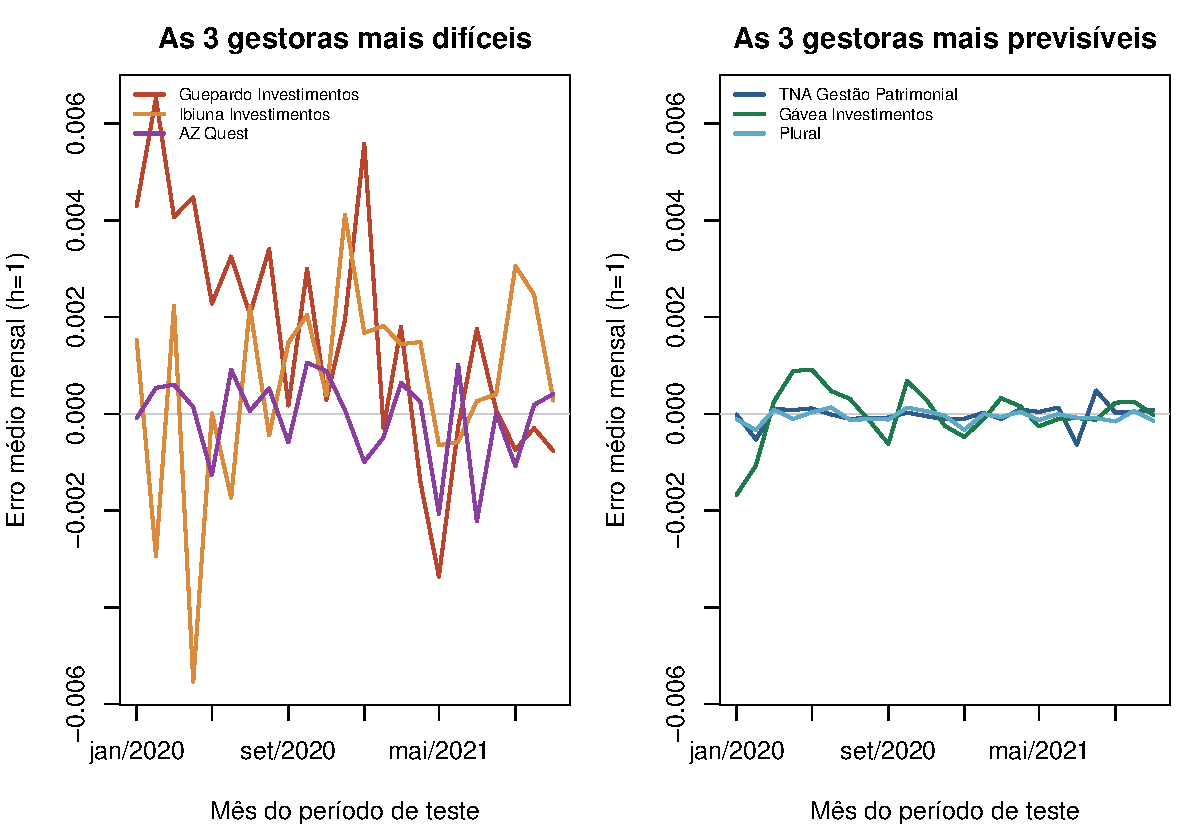
\includegraphics[width=\linewidth]{fig_dinamica_erro_gestora_extremos.pdf}

\vspace{0.1em}
\scriptsize
Erro médio mensal fora da amostra, $h=1$. À esquerda, as três gestoras mais difíceis de
prever; à direita, as três mais previsíveis. Mesma escala nos dois painéis.
\end{column}

\begin{column}{0.41\textwidth}
\small
Entre as 40 gestoras, o erro varia quase trinta vezes, de $0{,}00050$ a $0{,}01424$.

\vspace{0.6em}
E não é ruído. Dividindo o teste ao meio, cada gestora se parece consigo mesma, com
correlação de $0{,}85$ na dispersão do erro. Quem é difícil em 2020 continua difícil em
2021.

\vspace{0.6em}
O viés, ao contrário, quase não importa: responde por menos de $0{,}5\%$ do erro quadrático,
e corrigi-lo melhora o RMSE em $0{,}04\%$. É a variância que precisa ser explicada.
\end{column}
\end{columns}

\end{frame}

% ---------------------------------------------------------------- 8
\begin{frame}{Erro e margem por gestora, nos quatro horizontes}

\centering
\scriptsize
\setlength{\tabcolsep}{3.2pt}
\begin{tabular}{@{}lr rrrr rrrr@{}}
\toprule
& & \multicolumn{4}{c}{RMSE fora da amostra} & \multicolumn{4}{c}{Margem sobre a ingênua (\%)} \\
\cmidrule(lr){3-6}\cmidrule(lr){7-10}
Gestora & Fundos & $h{=}1$ & $h{=}3$ & $h{=}6$ & $h{=}12$ & $h{=}1$ & $h{=}3$ & $h{=}6$ & $h{=}12$ \\
\midrule
Guepardo & 11 & $0{,}01424$ & $0{,}02305$ & $0{,}03358$ & $0{,}05649$ & $1{,}2$ & $1{,}0$ & $-0{,}1$ & $-1{,}3$ \\
Ibiuna & 7 & $0{,}01331$ & $0{,}02131$ & $0{,}02492$ & $0{,}02848$ & $3{,}1$ & $6{,}8$ & $8{,}2$ & $14{,}3$ \\
AZ Quest & 22 & $0{,}01092$ & $0{,}01461$ & $0{,}01650$ & $0{,}01871$ & $3{,}1$ & $6{,}7$ & $9{,}5$ & $15{,}1$ \\
Squadra & 15 & $0{,}01069$ & $0{,}01588$ & $0{,}02090$ & $0{,}03058$ & $-5{,}4$ & $-13{,}7$ & $-24{,}3$ & $-45{,}6$ \\
Núcleo Capital & 22 & $0{,}01037$ & $0{,}01810$ & $0{,}02468$ & $0{,}03538$ & $-1{,}0$ & $-2{,}1$ & $-2{,}0$ & $-5{,}7$ \\
\midrule
\multicolumn{10}{c}{\textit{trinta gestoras intermediárias omitidas}} \\
\midrule
Itaú & 466 & $0{,}00261$ & $0{,}00385$ & $0{,}00473$ & $0{,}00559$ & $1{,}9$ & $4{,}2$ & $6{,}2$ & $8{,}1$ \\
Dahlia Capital & 18 & $0{,}00245$ & $0{,}00422$ & $0{,}00549$ & $0{,}00631$ & $2{,}4$ & $5{,}3$ & $8{,}0$ & $10{,}2$ \\
TNA & 29 & $0{,}00150$ & $0{,}00216$ & $0{,}00278$ & $0{,}00384$ & $0{,}1$ & $-0{,}8$ & $-0{,}8$ & $2{,}3$ \\
Gávea & 17 & $0{,}00144$ & $0{,}00265$ & $0{,}00365$ & $0{,}00472$ & $2{,}2$ & $4{,}2$ & $7{,}9$ & $10{,}4$ \\
Plural & 1 & $0{,}00050$ & $0{,}00079$ & $0{,}00104$ & $0{,}00134$ & $-2{,}4$ & $-3{,}7$ & $-2{,}8$ & $-6{,}1$ \\
\bottomrule
\end{tabular}

\vspace{0.8em}
\raggedright
\small
As cinco mais difíceis e as cinco mais previsíveis, de 40 grupos de gestora, ordenadas por
RMSE em $h=1$. Erro alto e margem baixa não são a mesma coisa: a AZ Quest é das mais
difíceis e ainda assim o modelo ajuda $15{,}1\%$ nela em $h=12$, enquanto a Squadra é o único
caso em que o modelo piora de forma expressiva e crescente com o horizonte.

\end{frame}

% ---------------------------------------------------------------- 9
\begin{frame}{O que explica a variância: concentração}

\begin{columns}[T]
\begin{column}{0.53\textwidth}
\scriptsize
\begin{tabular}{@{}lrrc@{}}
\toprule
Variável & Coef. & $t$ & Sig. \\
\midrule
Intercepto & $-0{,}0122$ & $-1{,}07$ & n.s. \\
Beta médio da cota & $0{,}0015$ & $0{,}55$ & n.s. \\
Tamanho médio & $0{,}0009$ & $1{,}34$ & n.s. \\
Cotistas médio & $0{,}0001$ & $0{,}18$ & n.s. \\
Proporção de fundos de cotas & $-0{,}0006$ & $-0{,}31$ & n.s. \\
Fluxo médio sobre patrimônio & $-0{,}0092$ & $-1{,}38$ & n.s. \\
Concentração média da carteira & $0{,}0736$ & $3{,}76$ & $1\%$ \\
\midrule
$R^2$ & \multicolumn{3}{r}{$0{,}496$} \\
\bottomrule
\end{tabular}

\vspace{0.5em}
\scriptsize
Variável dependente: desvio-padrão do erro fora da amostra de cada uma das 40 gestoras,
medido só no teste. Explicativas medidas só no treino.
\end{column}

\begin{column}{0.45\textwidth}
\small
Com todas as seis características juntas, a concentração é a única significativa, e o
modelo explica metade da variação entre casas.

\vspace{0.7em}
Descendo ao nível de fundo e mês, a correlação entre concentração e erro é:

\vspace{0.3em}
\centering
\begin{tabular}{@{}lr@{}}
\toprule
Contemporânea & $0{,}48$ \\
Defasada em um mês & $0{,}49$ \\
Dentro do mesmo fundo & $0{,}07$ \\
\bottomrule
\end{tabular}

\vspace{0.6em}
\raggedright
As duas primeiras quase iguais afastam coincidência de mesmo mês. A terceira, perto de zero,
mostra que a concentração diferencia fundos entre si, e não meses de um mesmo fundo. É um
traço permanente, não um sinal de curto prazo.
\end{column}
\end{columns}

\end{frame}

% ---------------------------------------------------------------- 10
\begin{frame}{Conclusão}

\begin{itemize}
  \item Beta da cota e concentração do resto da carteira explicam o peso de forma
        consistente. Tamanho e fluxo, quase nada.
  \item O ajuste ao alvo é positivo mas lento, com meia-vida de dez meses, e ainda assim
        bate a previsão ingênua nos quatro horizontes testados.
  \item A dificuldade de prever é heterogênea, persistente e explicada pela concentração
        da carteira. Essa é a regularidade nova do trabalho.
\end{itemize}

\vspace{0.9em}
\textbf{Limitações}

\begin{itemize}
  \item Metade da variância do erro entre gestoras segue sem explicação.
  \item O beta é medido no próprio mês, e não defasado como as demais características.
  \item $d_{i,n,t}$ e $\Delta w$ compartilham $-w_{i,n,t}$, o que favorece mecanicamente
        $\widehat\lambda>0$.
  \item A amostra termina em 2021.
\end{itemize}

\end{frame}

\end{document}
